\documentclass[12pt]{article}
\usepackage[hmargin={1in},vmargin={1in,1in},foot={.6in}]{geometry}   
\geometry{letterpaper} 
\usepackage{helvet}
\renewcommand{\familydefault}{\sfdefault}    
%\geometry{landscape}          
%\usepackage[parfill]{parskip}
\usepackage{color,graphicx}
%\usepackage{covington}
%\usepackage{xyling}
\usepackage{setspace}
\usepackage{amsmath}
\usepackage{amssymb}
%\usepackage{graphicx,color}
%\usepackage{theorem}
%\usepackage{tabularx}
%\usepackage{subfig}
%\usepackage{vowel}
%\usepackage{mathrsfs}
%\usepackage{varioref}
%\usepackage{textcomp}
%\usepackage{avm}
%\usepackage{textcomp}
%\usepackage{mflogo}
%\usepackage{wasysym}
%\usepackage{pstricks, pst-plot, pst-node, pst-tree, colortab}
%\usepackage{qtree}
 %\usepackage{tree-dvips}
% \usepackage{linguex}
\usepackage{gb4e}
 \usepackage{multirow}
% \usepackage[stable]{footmisc}
% \usepackage{pifont}
%\usepackage{todonotes}
%\usepackage{natbib}
\usepackage{apacite}
%\usepackage[normalem]{ulem}
\usepackage[font=footnotesize,labelfont=bf]{caption}

 %\setlength{\parskip}{.55ex plus 0.1ex}


\usepackage{fancyhdr} % This should be set AFTER setting up the page geometry
\pagestyle{plain} % options: empty , plain , fancy
\lhead{}\chead{}\rhead{}
\renewcommand{\headrulewidth}{.3pt}
\lfoot{}\cfoot{\thepage}\rfoot{}
%\renewcommand{\footrulewidth}{.3pt}
\newcommand{\txtp}{\textipa}
\renewcommand{\rm}{\textrm}
\newcommand{\sem}[1]{\mbox{$[\![$#1$]\!]$}}
\newcommand{\lam}{$\lambda$}
\newcommand{\lan}{$\langle$}
\newcommand{\ran}{$\rangle$}
\newcommand{\type}[1]{\ensuremath{\left \langle #1 \right \rangle }}
\newcommand{\defeq}{$\mathrel{\mathop:}=$ }
\renewcommand{\and}{$\wedge$ }


%\renewcommand{\Extopsep}{2pt}


\newcommand{\bex}{\begin{examples}}
\newcommand{\eex}{\end{examples}}

%bullet points
\newcommand{\bit}{\begin{itemize}}
\newcommand{\eit}{\end{itemize}}

%numbering, non sequential
\newcommand{\ben}{\begin{enumerate}}
\newcommand{\een}{\end{enumerate}}

\renewcommand{\abstractname}{The goal:}


\definecolor{Red}{RGB}{255,0,0}
\newcommand{\red}[1]{\textcolor{Red}{#1}}


\begin{document}

\begin{center}\textbf{When ``all" means not all: nonliteral interpretations of universal quantifiers}\\*[5pt]
\end{center}

%\vspace{-11pt}

A great deal of research has examined informativeness-based accounts of scalar implicature, such as strengthening ``some" to mean \emph{not all} \shortcite{gazdar1979pragmatics, degen2014processing}. Less well studied, on the other hand, is the converse effect in which ``all" is relaxed to produce nonliteral interpretations such as \emph{a lot but not all}. For example, ``All of the people in the audience laughed" means that many (but possibly not all) of the people in the audience laughed, and ``Bob took all of the credit" means that Bob took more credit than he deserved, and the speaker is upset about it. This introduces a nonliteral interpretation of ``all" that in fact contradicts its literal semantics. Recent work has shown that modeling language understanding as reasoning about the speaker's communicative goal can produce hyperbolic interpretations as well as relevant affective subtexts \shortcite{kao2014nonliteral}. Here we describe two experiments that explore listeners' interpretations of ``all" in different contexts. We then present a computational model that predicts these interpretations by reasoning about informativeness with respect to the speaker's communicative goal.
%\subsection*{Behavioral Experiments}

\textbf{Experiment 1} examines the effect of prior knowledge on interpretations of ``all." In Experiment 1a, 60 participants on Mechanical Turk read scenarios in which a character (Ann) brought 10 M\&M�s, cookies, or pies to a party. Participants rated how likely it is that another character (Bob) ate certain amounts of the food items. In Experiment 1b, 40 participants read scenarios in which Ann said to a friend, ``Bob ate some/all of the M\&M's/cookies/pies!" Participants rated how likely it is that Bob ate certain amounts of the food items give Ann's utterance. Results suggest that the ``all" in Ann's utterance is more likely to be interpreted hyperbolically when its literal meaning is increasingly unlikely under the prior distribution ($\beta$=.04, $SE$=.02, $t$=2.45, $p$$<$.05). 

\textbf{Experiment 2} examines the affect communicated with hyperbolic uses of ``all". In Experiment 2a, 40 participants rated how Ann feels given that Bob ate certain amounts of the items; in general, Ann feels more negative the more items Bob eats ($\beta$=.06, $SE$=.003, $t$=20.1, $p$$<$.0001). In Experiment 2b, 60 participants rated how Ann feels given that Bob ate certain amounts \emph{and} that she said: ``Bob ate some/all of the M\&M's/cookies/pies!" Even when Bob did not eat all of the items, participants rate Ann as feeling more negative when she says ``all" than when she says ``some" ($\beta$=.31, $SE$=.04, $t$=7.7, $p$$<$.0001, Fig.~2). This suggests that hyperbolic uses of ``all" convey additional affect.


%\begin{figure}[h!]
%%\scalebox{0.8}{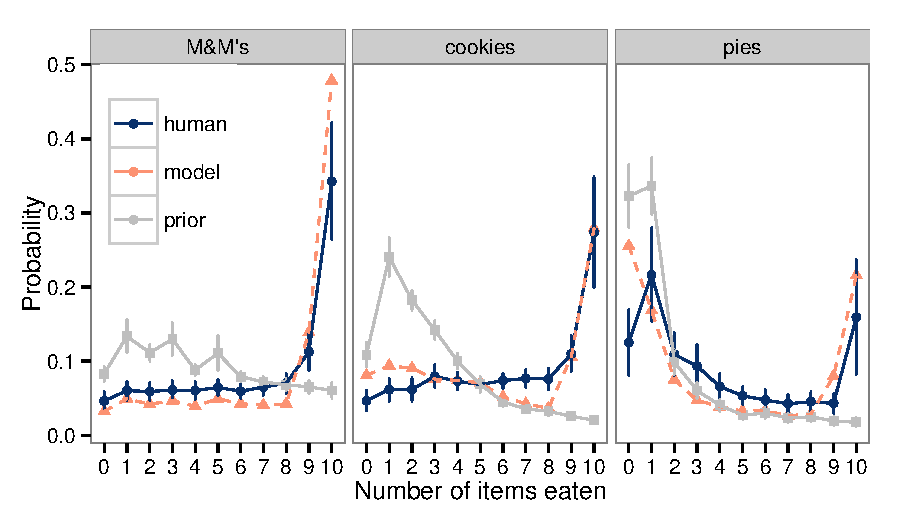
\includegraphics{figure1.pdf}}
%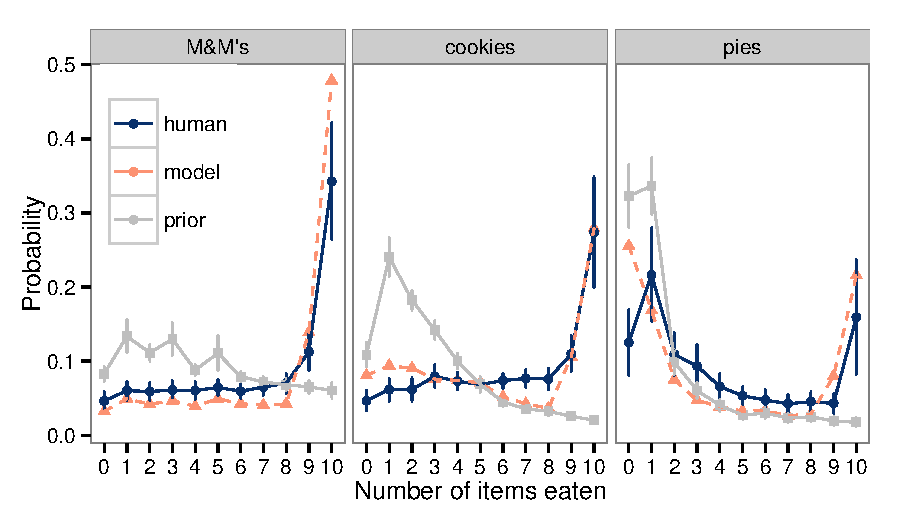
\includegraphics[width=12cm, height=5cm]{figure1.pdf}
%\caption{Gray lines (prior) show prior probabilities of Bob eating various amounts of food items given the three food types; blue lines (human) shows participants' interpretations of ``all" given different food types; pink lines (model) shows model predictions. The model predictions closely match human data (r=0.91).}
%\end{figure}

To explain the nonliteral interpretation of the universal quantifier ``all," we present an extension to the \textbf{Rational Speech Act model} \cite{frank2012predicting} and introduce the idea that a speaker may have multiple possible communicative goals. For example, Ann may want to communicate how many items Bob ate, \emph{or} how she feels about Bob's behavior. If Ann wants to communicate negative feelings about Bob to a literal listener, saying ``Bob ate all of the pies" will achieve this effect, since the literal listener will believe that Bob ate all 10 pies, which is associated with high negative affect. A pragmatic listener, however, reasons about background knowledge as well as Ann's communicative goal. The pragmatic listener knows that it is highly unlikely for Bob to have eaten all 10 pies, but that it is likely for Ann to want to communicate negative affect about Bob and not necessarily how many pies he ate. As a result, the pragmatic listener will infer that Bob ate \emph{some} of the pies, but that Ann feels negative about it. 

%\begin{figure}[h!]
%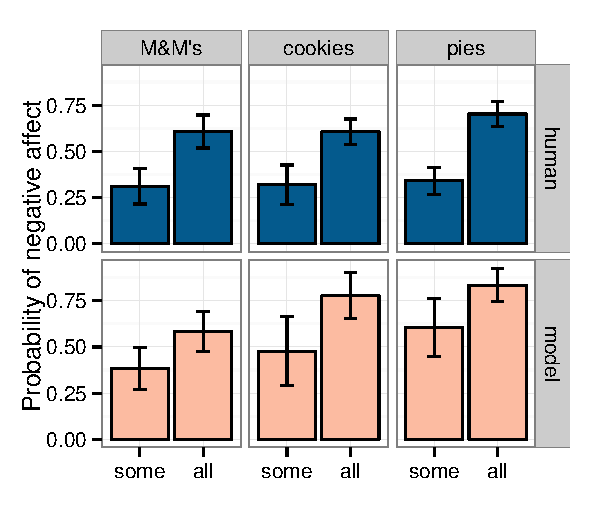
\includegraphics[width=8cm, height=5cm]{figure2.pdf}
%%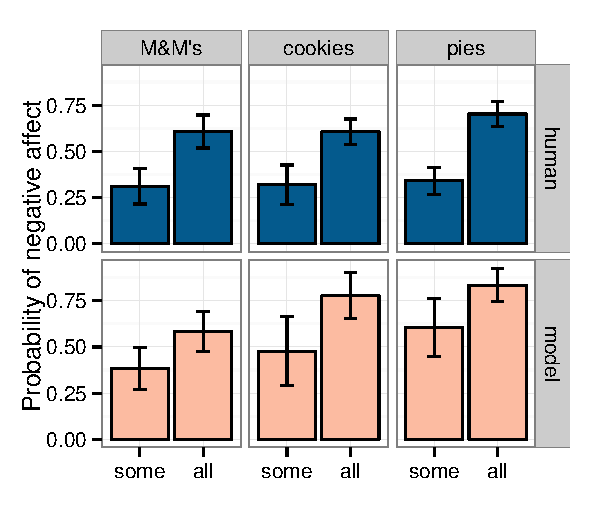
\includegraphics[width=6.5cm, height=4cm]{figure2.pdf}
%\caption{Negative affect conveyed in literal ``some" v.s. hyperbolic ``all." Human data and model both show that hyperbolic uses of ``all" convey significantly more affect than literal uses of ``some."}
%\label{figure}
%\end{figure}

Using the priors from Experiment 1a and Experiment 2a, the model produces interpretations that closely match humans' (r=0.91) (Fig. 1). Moreover, the model infers additional affect from hyperbolic uses of ``all" (Fig. 2), successfully capturing the rhetorical effect of hyperbole.  This suggests that by incorporating prior background knowledge, linguistic information, and reasoning about the speaker's communicative goals, the model is able to recover the intended meaning of a nonliteral utterance. Taking together the empirical results and model predictions, we discuss implications on the role of prior knowledge and pragmatic reasoning in language understanding as well as how these factors shape the social and affective information conveyed through nonliteral language.

\begin{figure}[h]
\begin{minipage}[b]{.6\textwidth}
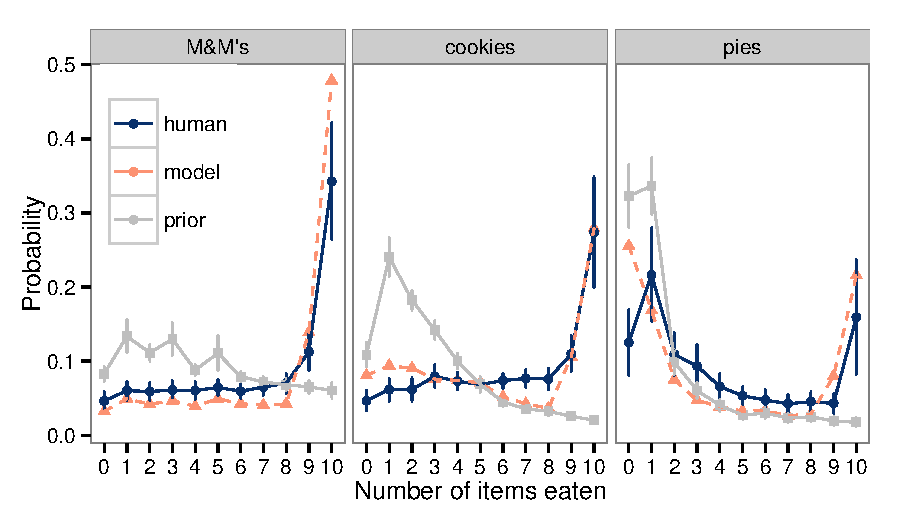
\includegraphics[width=10cm, height=4.5cm]{figure1.pdf}
%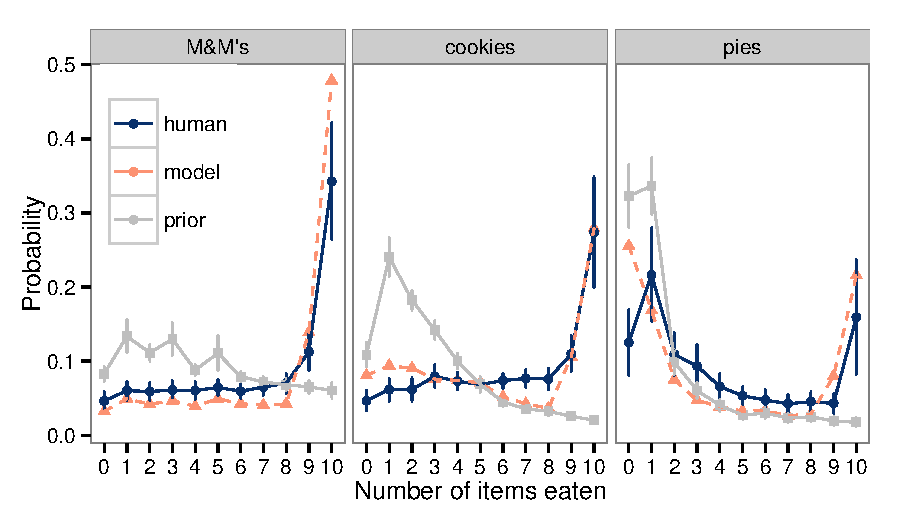
\includegraphics[width=10cm, height=4cm]{figure1.pdf}
\caption{Gray lines (prior) show prior probabilities of Bob eating various amounts of food items given the three food types; blue lines (human) shows participants' interpretations of ``all" given different food types; pink lines (model) shows model predictions. The model predicts closely match human data (r=0.91).}
\end{minipage}
\begin{minipage}[b]{.4\textwidth}
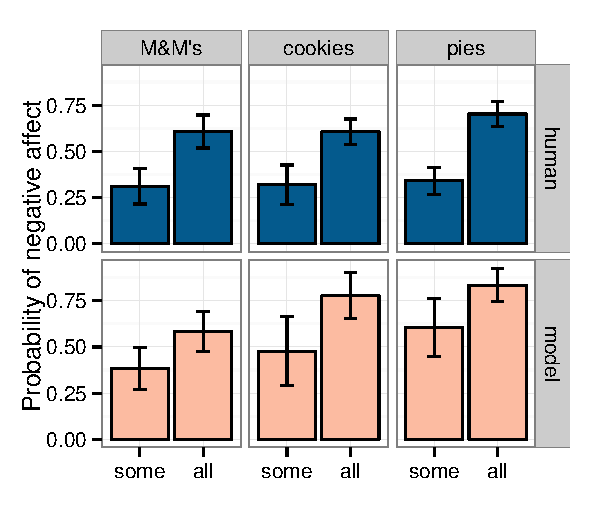
\includegraphics[width=6.5cm, height=4.5cm]{figure2.pdf}
%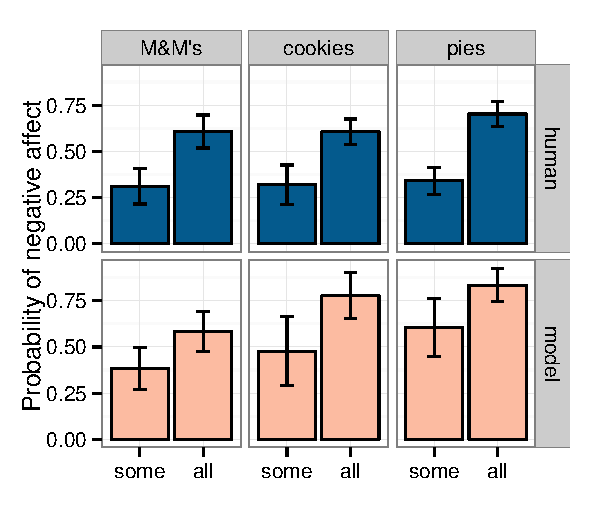
\includegraphics[width=6.5cm, height=4cm]{figure2.pdf}
\caption{Negative affect conveyed in literal ``some" v.s. hyperbolic ``all." Human data and model both show that hyperbolic uses of ``all" convey more affect than literal uses of ``some."}
\end{minipage}
\label{figure}
\end{figure}
%In order to recover the intended nonliteral meaning, a pragmatic listener needs to incorporate linguistic information, background knowledge, and the speaker's communicative goal. 


%\newpage

\bibliographystyle{chicago}
\bibliography{all.bib}




\end{document}